% 66-33(66쪽) — 두 원 $x^{2}+y^{2}=8$, $x^{2}+y^{2}=20$ 과 직선 $y=2$ 가 만나는 점 $\pt{P}$, $\pt{Q}$ 그리고 점 $\pt{A}$(원문 「오른쪽 그림」). 스캔 화질이 낮아 TikZ 로 다시 그림.
% 라벨은 원문 것만: $\pt{P}$, $\pt{Q}$, $\pt{A}$, $\pt{O}$, $y=2$, 두 원의 방정식, $\alpha$, $\beta$.
% $\cos\alpha\sin\beta$ 의 값(답)이 읽히지 않게 좌표 눈금·각의 크기는 적지 않는다.
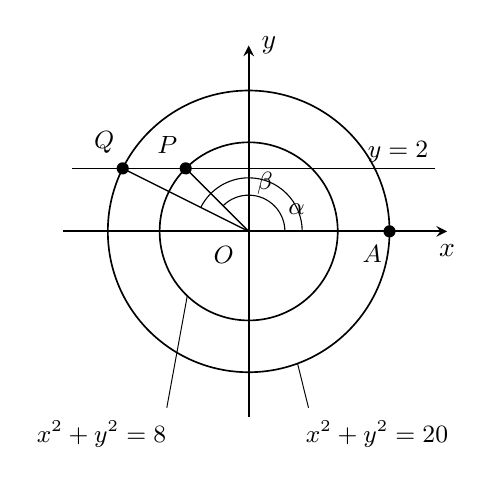
\begin{tikzpicture}[line width=0.6pt, x=0.40cm, y=0.40cm, >=stealth]
  \draw[->, line width=0.7pt] (-5.9,0) -- (6.3,0) node[below=1pt] {$x$};
  \draw[->, line width=0.7pt] (0,-5.9) -- (0,5.9) node[right=1pt] {$y$};
  \draw (0,0) circle (2.828);
  \draw (0,0) circle (4.472);
  \draw[line width=0.5pt] (-5.6,2) -- (5.9,2) node[anchor=south east, font=\small, inner sep=2pt] {$y=2$};
  \draw[line width=0.5pt] (0,0) -- (-2,2);
  \draw[line width=0.5pt] (0,0) -- (-4,2);
  \draw[line width=0.4pt] (1.15,0) arc (0:135:1.15);
  \draw[line width=0.4pt] (1.70,0) arc (0:153.435:1.70);
  \fill (-2,2) circle (2.2pt);
  \fill (-4,2) circle (2.2pt);
  \fill (4.472,0) circle (2.2pt);
  \node[font=\small] at (1.52,0.72) {$\alpha$};
  \node[font=\small] at (0.52,1.52) {$\beta$};
  \node[anchor=south east, font=\small] at (-1.95,2.15) {$\pt{P}$};
  \node[anchor=south east, font=\small] at (-3.95,2.15) {$\pt{Q}$};
  \node[anchor=north east, font=\small] at (4.55,-0.12) {$\pt{A}$};
  \node[anchor=north east, font=\small] at (-0.15,-0.15) {$\pt{O}$};
  \draw[line width=0.35pt] (-2.6,-5.6) -- (-1.95,-2.05);
  \draw[line width=0.35pt] (1.9,-5.6) -- (1.55,-4.19);
  \node[anchor=north east, font=\small] at (-2.3,-5.7) {$x^{2}+y^{2}=8$};
  \node[anchor=north west, font=\small] at (1.5,-5.7) {$x^{2}+y^{2}=20$};
\end{tikzpicture}
